% figures/library-case.tex
\documentclass[11pt]{article}
\usepackage[margin=1.5cm]{geometry}
\usepackage{tikz}
\usetikzlibrary{positioning,shapes.geometric,arrows.meta,calc}
\pagestyle{empty}
\begin{document}
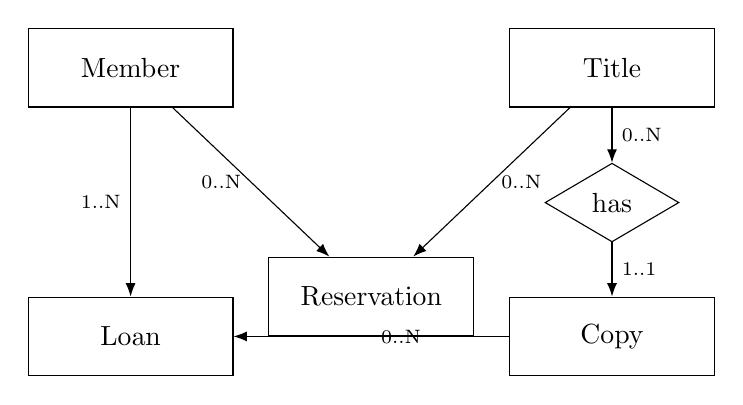
\begin{tikzpicture}[node distance=18mm, >=Latex]
  \node[draw, rectangle, minimum width=2.6cm, minimum height=1cm] (Member) {Member};
  \node[draw, rectangle, minimum width=2.6cm, minimum height=1cm, right=35mm of Member] (Title) {Title};
  \node[draw, rectangle, minimum width=2.6cm, minimum height=1cm, below=24mm of Title] (Copy) {Copy};
  \node[draw, rectangle, minimum width=2.6cm, minimum height=1cm, below=24mm of Member] (Loan) {Loan};
  \node[draw, rectangle, minimum width=2.6cm, minimum height=1cm, below=24mm of $(Member)!0.5!(Title)$] (Res) {Reservation};

  \node[draw, diamond, aspect=2, minimum width=1.6cm, minimum height=1cm, below=7mm of Title] (Has) {has};

  \draw[->] (Title) -- (Has) node[midway, right, font=\scriptsize] {0..N};
  \draw[->] (Has) -- (Copy) node[midway, right, font=\scriptsize] {1..1};

  \draw[->] (Member) -- (Loan) node[midway, left, font=\scriptsize] {1..N};
  \draw[->] (Copy) -- (Loan) node[midway, right, font=\scriptsize] {0..N};

  \draw[->] (Member) -- (Res) node[midway, left, font=\scriptsize] {0..N};
  \draw[->] (Title) -- (Res) node[midway, right, font=\scriptsize] {0..N};
\end{tikzpicture}
\end{document}
